\id{МРНТИ \href{https://grnti.ru/?p1=52&p2=13&p3=07}{52.13.07}}{https://doi.org/10.58805/kazutb.v.4.25-554}
\begin{articleheader}

\sectionwithauthors{А.Ә. Қазбек, Д.К. Ахметканов, Е.Х. Абен, С.С. Мырзахметов}{ПОВЫШЕНИЕ КАЧЕСТВА ДРОБЛЕНИЯ РУДЫ ПРИ СКВАЖИННОЙ ОТБОЙКЕ С
ИСПОЛЬЗОВАНИЕМ ПРОГРАММЫ MICROMINE МЕСТОРОЖДЕНИЯ ЖОЛЫМБЕТ}

{\bfseries А.Ә. Қазбек, Д.К. Ахметканов\textsuperscript{\envelope }, Е.Х. Абен, С.С.
Мырзахметов}
\end{articleheader}
\begin{affiliation}
Satbayev University, Алматы, Казахстан

\raggedright {\bfseries \textsuperscript{\envelope }}Корреспондент-автор: \href{mailto:d.akhmetkanov@satbayev.university}{\nolinkurl{d.akhmetkanov@satbayev.university}}
\end{affiliation}

В ходе исследования, направленного на повышение качества дробления руды
при скважинной отбойке с использованием программы Micromine, возникли
некоторые вызовы, не зависящие от инженера по буровзрывным работам. В
частности, отсутствовала литологическая блочная модель, необходимая для
точного моделирования, которую геологическая служба не смогла
предоставить. Также геомеханический отдел сообщил о невозможности
составления блочной модели, а программное обеспечение ShotPlus не
поддерживало формат, предложенный для создания модели. Для решения
данных проблем изначально проводились исследования по оценке
возможностей улучшения параметров дробления руды при скважинном бурении.
В частности, исследование направлено на изучение эффективности программы
Micromine в условиях отсутствия литологической блочной модели и
невозможности использования ПО ShotPlus для создания геомеханической
модели. В связи с этим было принято решение о предоставлении информации
в письменной и графической формах после картирования. Несмотря на эти
ограничения, использование программы Micromine позволило достичь
улучшения параметров дробления руды.

Преимущества исследования включают оптимизацию сетки бурения и снижение
объемов буровых работ, что подтверждает эффективность выбранного
подхода. Однако следует критически рассмотреть и возможные недостатки,
такие как ограниченность применения методов без полноценной
литологической модели и несовместимость с другим программным
обеспечением.

{\bfseries Ключевые слова:} скважинное бурение, дробление руды, Micromine,
геомеханическая модель, ShotPlus, литологическая блочная модель.

\begin{articleheader}
{\bfseries ЖОЛЫМБЕТ КЕНОРНЫН MICROMINE БАҒДАРЛАМАСЫН ПАЙДАЛАНА ОТЫРЫП
ҰҢҒЫМАЛЫҚ УАТУ КЕЗІНДЕ КЕНДІ ҰСАҚТАУ САПАСЫН АРТТЫРУ}

{\bfseries А.Ә. Қазбек, Д.К. Ахметканов\textsuperscript{\envelope }, Е.Х. Абен, С.С.
Мырзахметов}
\end{articleheader}
\begin{affiliation}

Сәтбаев Университеті, Алматы, Қазақстан,

е-mail: \href{mailto:d.akhmetkanov@satbayev.university}{\nolinkurl{d.akhmetkanov@satbayev.university}}
\end{affiliation}

Зерттеу барысында Micromine бағдарламасын қолдану арқылы ұңғыма
жарылыстарымен кенді ұсақтау сапасын арттыруға бағытталған жұмыстар
жүргізілді. Бұл мақсатты жүзеге асыру барысында бұрғылау-жарылыс
жұмыстары инженері тәуелсіз кейбір қиындықтарға тап болды. Атап
айтқанда, геологиялық қызмет литологиялық блоктық модельді ұсына алмады,
ал геомеханикалық бөлім блоктық модель құрастыру мүмкін емес деп
мәлімдеді. Сонымен қатар, ShotPlus бағдарламалық жасақтамасы
геомеханикалық бөлімнің ойластырған форматындағы блоктық модельді
қолдамады, және ShotPlus өкілдері олардың бағдарламасы блоктық
геомеханикалық модель үшін арналмағанын хабарлады. Бұл мәселелерді шешу
үшін бастапқыда ұңғымалық бұрғылау кезінде кенді ұсақтау параметрлерін
жақсарту мүмкіндіктерін бағалау бойынша зерттеулер жүргізілді. Атап
айтқанда, зерттеу литологиялық блоктық модель болмаған жағдайда
Micromine бағдарламасының тиімділігін және геомеханикалық модель жасау
үшін ShotPlus қолданбасын пайдалану мүмкін .стігін зерттеуге
бағытталған. Қалыптасқан жағдайға байланысты геомеханикалық қызметтің
ақпаратын карталаудан кейін жазбаша және графикалық түрде ұсыну туралы
шешім қабылданды. Осы шектеулерге қарамастан, Micromine бағдарламасын
қолдану кенді ұсақтау параметрлерін жақсартуға мүмкіндік берді, бұл
технологияны қолданудың тиімділігін дәлелдейді.

Зерттеудің артықшылықтары бұрғылау торын оңтайландыруды және таңдалған
тәсілдің тиімділігін растайтын бұрғылау жұмыстарының көлемін азайтуды
қамтиды. Дегенмен, толық литологиялық модельсіз әдістерді қолданудың
шектелуі және басқа бағдарламалық құралмен үйлесімсіздік сияқты ықтимал
кемшіліктерді де сыни тұрғыдан қарастыру керек.

{\bfseries Түйін сөздер:} ұңғыма жарылыстары,кенді ұсақтау, Micromine,
геомеханикалық модель, ShotPlus, литологиялық блоктық модель.
\begin{articleheader}

{\bfseries IMPROVING THE QUALITY OF ORE CRUSHING DURING DOWNHOLE EXTRACTION
USING THE MICROMINE PROGRAM OF THE ZHOLYMBET DEPOSIT}

{\bfseries A. Kazybek, D. Akhmetkanov\textsuperscript{\envelope }, E. Aben, S.
Myrzakhmetov}
\end{articleheader}
\begin{affiliation}

Satbayev University, Almaty, Kazakhstan,

е-mail: \href{mailto:d.akhmetkanov@satbayev.university}{\nolinkurl{d.akhmetkanov@satbayev.university}}
\end{affiliation}

This study aimed to enhance ore fragmentation quality during blast hole
drilling using the Micromine software. During the implementation of this
goal, several challenges arose that were beyond the control of the
drilling and blasting engineer. Specifically, the absence of a
lithological block model from the geological department was a
significant obstacle. Furthermore, the geomechanical department reported
that creating a block model was not feasible, and the ShotPlus software
did not support the format initially intended by the geomechanical team.
ShotPlus representatives also confirmed that their software was not
designed for geomechanical block modeling. To solve these problems,
studies were initially conducted to assess the possibilities of
improving ore crushing parameters during downhole drilling. In
particular, the study is aimed at studying the effectiveness of the
Micromine program in the absence of a lithological block model and the
inability to use ShotPlus software to create a geomechanical model.
Given this situation, it was decided to provide the geomechanical
information in written and graphical forms after mapping. Despite these
limitations, the use of Micromine software allowed for improvements in
ore fragmentation parameters, confirming the effectiveness of this
technology.

The advantages of the study include optimization of the drilling grid
and reduction of drilling volumes, which confirms the effectiveness of
the chosen approach. However, possible disadvantages should also be
critically considered, such as the limited use of methods without a
full-fledged lithological model and incompatibility with other software.

{\bfseries Keywords:} blast hole drilling, ore fragmentation, Micromine,
geomechanical model, ShotPlus, lithological block model.
\begin{multicols}{2}

{\bfseries Введение}. В последние годы повышение эффективности дробления
руды при скважинной отбойке стало ключевой задачей для горнодобывающих
предприятий {[}1{]}. Это связано с необходимостью улучшения
экономических показателей и повышения качества конечного продукта.
Технологии моделирования, такие как программа Micromine, предлагают
возможности для оптимизации параметров буровзрывных работ (БВР). На
основе данной программы можно решать большой комплекс геологоразведочных
задач, возникающих при проектировании горнорудных предприятий. Наиболее
распространенными задачами являются статистический анализ геологической
информации, автоматизация процессов обработки и интерпретации данных
геологической разведки {[}2,3{]}. Однако внедрение этих технологий
сталкивается с рядом вызовов, включая отсутствие литологической блочной
модели и ограничения в использовании программного обеспечения,
предназначенного для создания геомеханических моделей {[}4,5{]}.

{\bfseries Материалы и методы.} Основной целью данного исследования
является оценка возможностей улучшения параметров дробления руды при
скважинном бурении, несмотря на существующие ограничения.

В рамках данного исследования использовались следующие методы и
инструменты:

1. Программное обеспечение: Основным инструментом для моделирования и
анализа данных стала программа Micromine. Micromine --- это
интегрированное программное обеспечение для геологического и
горнодобывающего моделирования, которое предоставляет инструменты для
анализа и визуализации геологических данных, проектирования рудников и
оптимизации процессов добычи. Сочетание геологического моделирования с
технологиями оптимизации делает Micromine мощным инструментом для
повышения эффективности подземных выемочных добычных единиц {[}6,7{]}.
Данная программа позволяет выполнять моделирование без необходимости
использования литологической блочной модели.

2. Процесс работы: Для моделирования и оптимизации параметров
буровзрывных работ была использована информация, полученная в результате
картирования и последующего анализа геомеханических данных. Поскольку
отсутствовала возможность создания полноценной блочной модели,
информация была предоставлена в письменной и графической формах, что
позволило корректировать параметры на основе фактических данных {[}8{]}.

3. Экспериментальные параметры: В процессе работы были произведены
расчеты линии наименьшего сопротивления для блока 270\_007, на основании
которых была разработана экспериментальная сетка бурения. Также были
учтены данные по отклонению фактических расположений пробуренных
скважин, что позволило провести корректировки в проектировании (рисунок
1,2,3).
\end{multicols}

\begin{figure}[H]
	\centering
	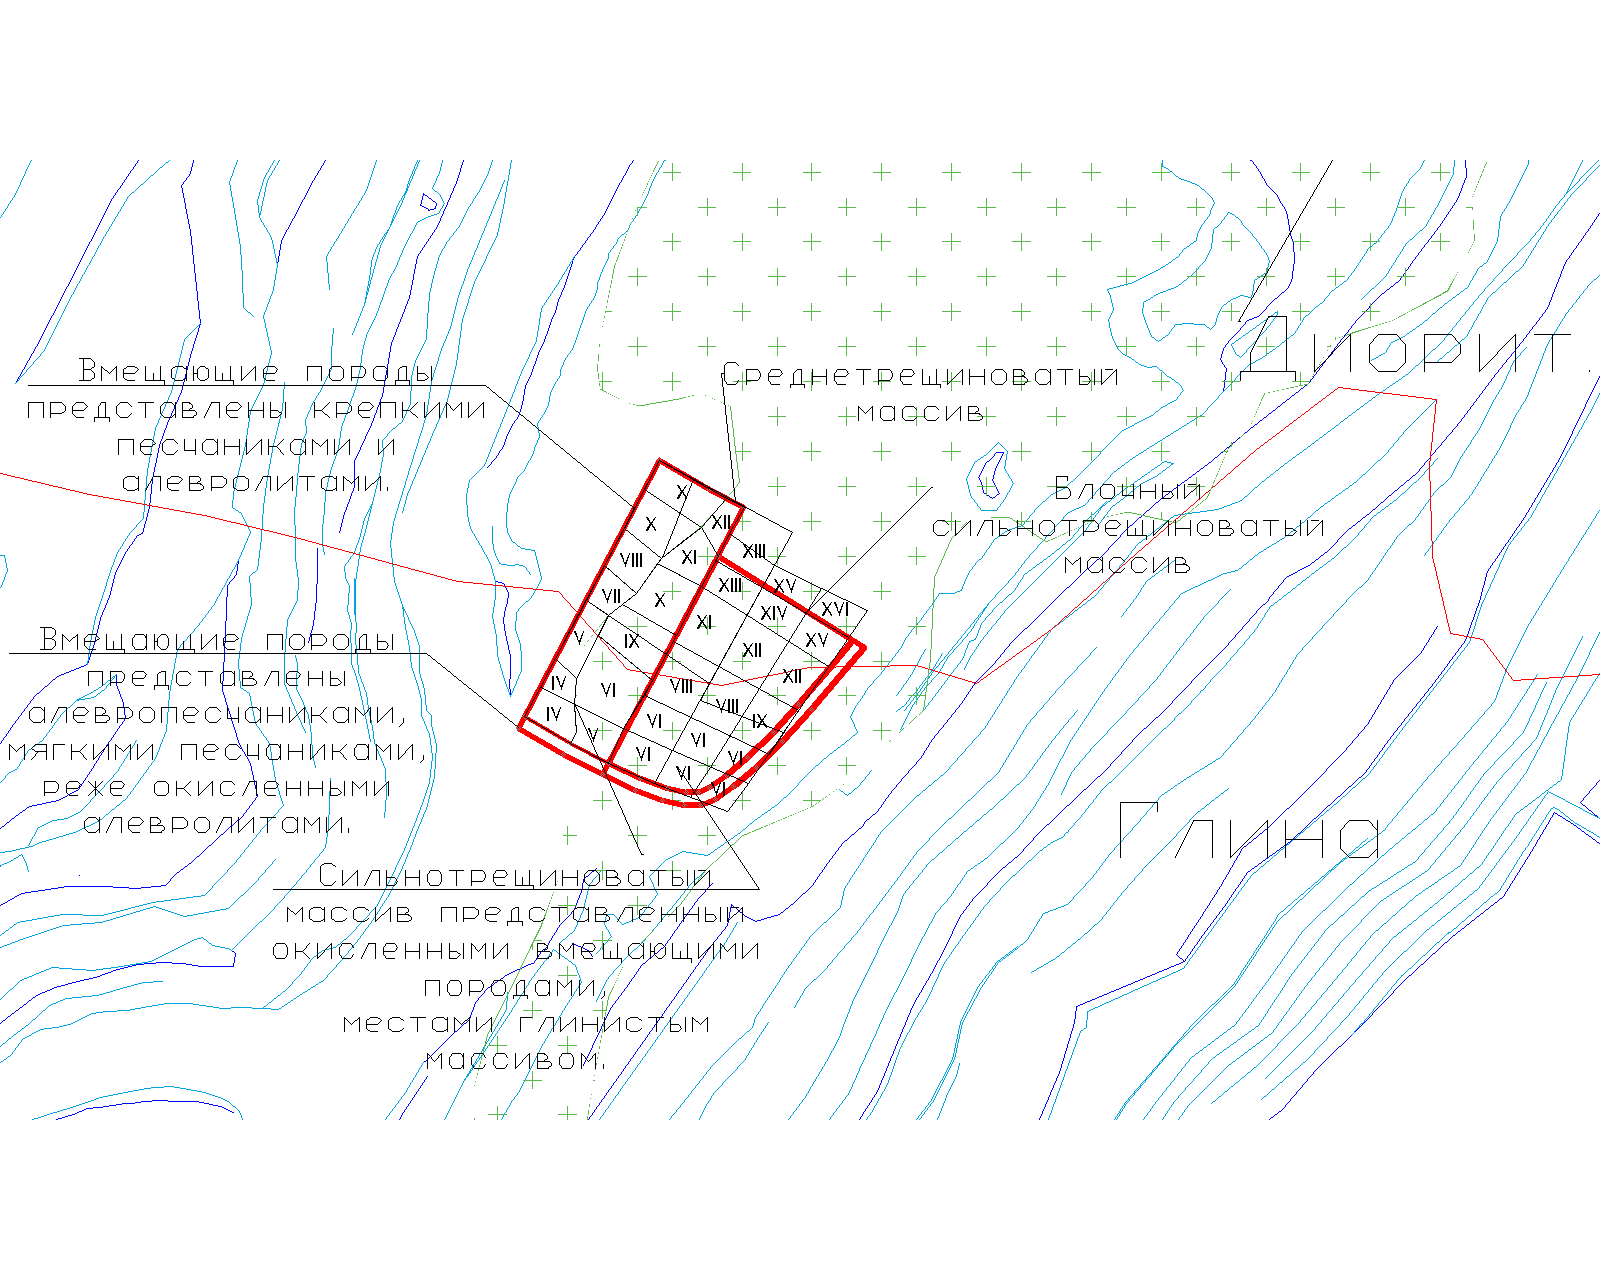
\includegraphics[width=0.8\textwidth]{media/gor/image27}
	\caption*{Рис. 1 -- Повышение уровня выполнения БВР и использование
	геотехнической блочной модели (при составлении БВР) для улучшения
	параметров карьера проекта Жолымбет}
\end{figure}

\begin{multicols}{2}

Одной из важнейших характеристик взрывных работ является расчетный
удельный расход ВВ, который зависит от свойств горной породы.

Для любой породы по категории трещиноватости и коэффициенту крепости f
расчетный удельный расход (qp, кг/м\textsuperscript{3}) ВВ для зарядов
рыхления при диаметре заряда определяется по формуле {[}9{]}:

\hspace{1em} qр = qэ . е . kd . ρ/2600, кг/м\textsuperscript{3} (1)

где qэ - эталонный расход граммонита 79/21 при кондиционном размере
кусков 500 мм, кг/м\textsuperscript{3} (таблица 1);

е - коэффициент работоспособности ВВ (таблица 2). Для упругих типов

ВВ е = 4316/Q, где Q -- удельная энергия применяемого ВВ, Дж/кг;

kd - поправочный коэффициент на допустимый размер куска (таблица 3);

ρ - плотность породы, кг/м\textsuperscript{3}.

\end{multicols}
\begin{longtable}[H]{|@{} 
  >{\centering\arraybackslash}p{(\columnwidth - 6\tabcolsep) * \real{0.40}}| % Adjusted first column
  >{\centering\arraybackslash}p{(\columnwidth - 6\tabcolsep) * \real{0.2}}| 
  >{\centering\arraybackslash}p{(\columnwidth - 6\tabcolsep) * \real{0.2}}| 
  >{\centering\arraybackslash}p{(\columnwidth - 6\tabcolsep) * \real{0.2}}|@{}}
\caption*{Таблица 1 - Эталонный расход ВВ при крепости породы}\\
\hline
\multirow{2}{*}{\shortstack[l]{Эталонный расход граммонита 79/21 \\ для кондиционного куска 0,5 м}} & 
\multicolumn{3}{c|}{Эталонный расход ВВ при крепости породы $f$, кг/м\textsuperscript{3}} \\ \cline{2-4}
& & & \\
Категория трещиноватости породы & 2 ÷ 5 & 6 ÷ 10 & 11 ÷ 20 \\ \hline
I & \textless{} 0,3 & \textless{} 0,35 & \textless{} 0,45 \\ 
II & 0,4 & 0,5 & 0,6 \\ 
III & 0,65 & 0,75 & 0,9 \\ 
IV & 0,85 & 1 & 1,2 \\ 
V & 1 & 1,2 & 1,4 \\ \hline
\end{longtable}


\begin{longtable}[H]{|@{} 
    >{\raggedright\arraybackslash}p{(\columnwidth - 6\tabcolsep) * \real{0.5165}}|
    >{\raggedright\arraybackslash}p{(\columnwidth - 6\tabcolsep) * \real{0.0644}}|
    >{\raggedright\arraybackslash}p{(\columnwidth - 6\tabcolsep) * \real{0.3547}}|
    >{\raggedright\arraybackslash}p{(\columnwidth - 6\tabcolsep) * \real{0.0644}}|@{}}
\caption*{Таблица 2 - коэффициент работоспособности ВВ} \\ \hline
Значение поправочного коэффициента е для различных ВВ & е & ВВ & e \\ \hline
\endfirsthead
Акватол М-15 & 0,76 & Акватол МГ & 0,93 \\
Граммонал А-45 & 0,79 & Акватол АВМ & 0,95 \\
Карбатол ГЛ-10В & 0,79 & Гранулит АС-4 (АС-4В) & 0,98 \\
Граммонал А-8 & 0,80 & Аммонит № 6ЖВ & 1,00 \\
Аммонит скальный N1 & 0,80 & Граммонит 79/21 & 1,00 \\
Аммонал скальный N3 & 0,80 & Ифзанит Т-80 & 1,08 \\
Детонит М & 0,82 & Граммонал А-50 & 1,10 \\
Алюмотол & 0,83 & Ифзанит Т-60 & 1,10 \\
Гранулит АС-8 (АС-8В) & 0,89 & Гранулит М & 1,13 \\
Аммонал водоустойчивый & 0,90 & Игданит & 1,13 \\
 &  & Гранулотол & 1,20 \\ \hline
\end{longtable}

\begin{longtable}[H]{|@{}
	>{\raggedright\arraybackslash}p{(\columnwidth - 12\tabcolsep) * \real{0.2671}}|
	>{\raggedright\arraybackslash}p{(\columnwidth - 12\tabcolsep) * \real{0.1221}}|
	>{\raggedright\arraybackslash}p{(\columnwidth - 12\tabcolsep) * \real{0.1221}}|
	>{\raggedright\arraybackslash}p{(\columnwidth - 12\tabcolsep) * \real{0.1221}}|
	>{\raggedright\arraybackslash}p{(\columnwidth - 12\tabcolsep) * \real{0.1221}}|
	>{\raggedright\arraybackslash}p{(\columnwidth - 12\tabcolsep) * \real{0.1221}}|
	>{\raggedright\arraybackslash}p{(\columnwidth - 12\tabcolsep) * \real{0.1221}}|@{}}
\caption*{Таблица 3 - поправочный коэффициент на допустимый размер куска} \\ 
\hline
  \endfirsthead
  \hline
  \endhead
  \hline
  \endfoot
  \endlastfoot
  Поправочный коэффициент на допустимый размер куска (dmax) Допустимый размер куска dmax, м & 0,250 & 0,500 & 0,750 & 1,0 & 1,25 & 1,5 \\ \hline
  kd & 1,3 & 1,0 & 0,85 & 0,75 & 0,7 & 0,65 \\ \hline
  \end{longtable}
  
  \begin{multicols}{2}

1. Удельный расход при крепости 10-12 и средней трещиноватости массива.

\(qp = 0,9*1,2*1,0*\frac{2710}{2600} = 1,125кг/м\)\textsuperscript{3}

2. Удельный расход при крепости 8-10 и средней трещиноватости массива.

\(qp = 0,75*1,2*1,0*\frac{2520}{2600} = 0,8723кг/м\)\textsuperscript{3}

3. Удельный расход при крепости 5-8 и сильной трещиноватости массива.

\(qp = 0,5*1,2*1,0*\frac{2520}{2600} = 0,58кг/м\)\textsuperscript{3}

По выбранным значениям диаметра заряда (dз), расчетного удельного
расхода ВВ вычисляются параметры скважинных зарядов.

\begin{enumerate}
\def\labelenumi{\arabic{enumi}.}
\item
  Вместимость 1 м скважины рассчитывается по формуле:
\end{enumerate}

$P = \frac{\pi \cdot d_3^2}{4} \cdot \Delta$, 

где Δ - плотность ВВ в скважине, кг/м\textsuperscript{3} .

Р=3,14*0,13*0,13*850/4=11,28 кг/м\textsuperscript{3}

2. Предельная линия сопротивления по подошве уступа W\textsubscript{n}
определяется по формулам:

\(Wn = 0.9\sqrt{\frac{P}{qp}}\) , \(Wn = 24d\sqrt{\frac{\Delta}{qp}}\)

2.1 Предельная линия сопротивления по подошве уступа W\textsubscript{n}
при крепости 10-12 и средней трещиноватости массива

\[Wn = 0.9\sqrt{\frac{11,28}{1,125}\ } = 2,85\ м\]

2.2 Предельная линия сопротивления по подошве уступа W\textsubscript{n}
при крепости 8-10 и средней трещиноватости массива

\(Wn = 0.9\sqrt{\frac{11,28}{0,8723}\ } = 3,24\ м\)

2.3 Предельная линия сопротивления по подошве уступа W\textsubscript{n}
при крепости 5-8 и сильной трещиноватости массива

\[Wn = 0.9\sqrt{\frac{11,28}{0,58}\ } = 5,79\ м\]

3. В зависимости от величины Wn определяется расстояние между скважинами
в ряду между парами парносближенных скважин первого ряда а (м) и между
рядами скважин b (м):

а = mWn, b = (0,8÷1)Wn,

где m = 0,8÷1,1 для вертикальных скважин;

m = 0,9÷1,3 для наклонных скважин.

Для данного блока принимаются следующие расстояния между скважинами в
ряду:

а= 3,3 м

а= 3,6 м

а= 3,8 м

а= 4,0 м

Расстояния между рядами скважин:

b= 2,7 м

b= 3,0 м

При применении в первом ряду парносближенных скважин расстояние между
скважинами во втором и последующих рядах и между рядами скважин
определяют в зависимости от Wn вычисленной для условий одиночной
скважины.

Получив все параметры БВР расчетным методом, далее проектируем в
Micromine проект на бурение блока (таблица 4). Так же продемонстрировано
отклонение фактических расположении пробуренных скважин {[}10,11,12{]}
\end{multicols}


\begin{figure}[H]
	\centering
	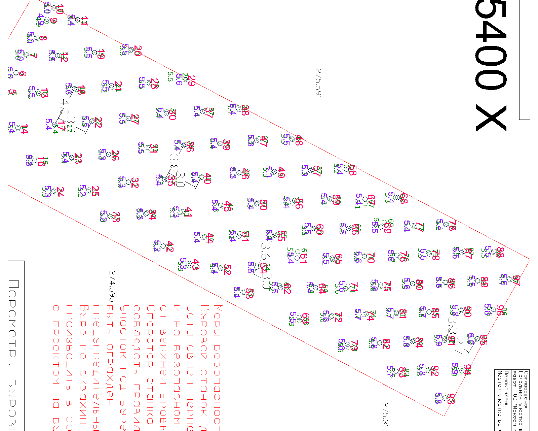
\includegraphics[width=0.8\textwidth]{media/gor/image29}
	\caption*{Рис. 2 - Проект массового взрыва блок 270-007}
\end{figure}


\begin{figure}[H]
	\centering
	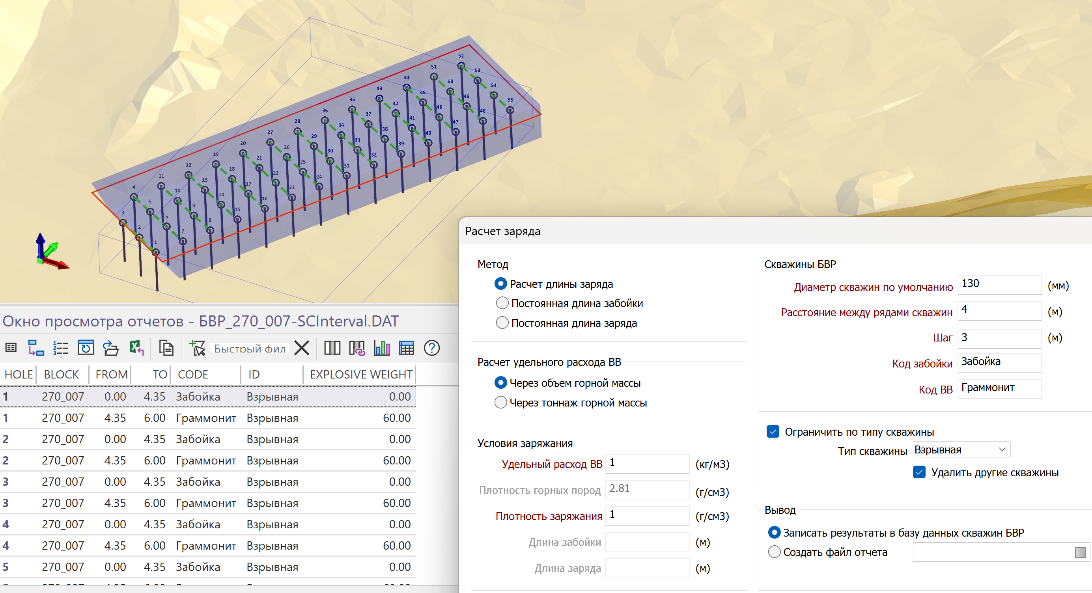
\includegraphics[width=0.8\textwidth]{media/gor/image30}
	\caption*{Рис. 3 - Создание схемы скважин БВР по полигону}
\end{figure}

\begin{longtable}[H]{|@{} 
	>{\centering\arraybackslash}p{(\columnwidth - 8\tabcolsep) * \real{0.3398}}| 
	>{\centering\arraybackslash}p{(\columnwidth - 8\tabcolsep) * \real{0.0971}}| 
	>{\centering\arraybackslash}p{(\columnwidth - 8\tabcolsep) * \real{0.2593}}| 
	>{\centering\arraybackslash}p{(\columnwidth - 8\tabcolsep) * \real{0.1889}}| 
	>{\centering\arraybackslash}p{(\columnwidth - 8\tabcolsep) * \real{0.1150}}|@{}}
\caption*{Таблица 4 -- Сравнительная таблица результатов проведенных
буровзрывных работ} \\ 
	\hline
  {\bfseries Наименование} & \begin{minipage}[b]{\linewidth}\centering
  {\bfseries Ед. изм.}
  \end{minipage} & \begin{minipage}[b]{\linewidth}\centering
  {\bfseries Проект стандартный, без использование геотехнических данных}
  \end{minipage} & \begin{minipage}[b]{\linewidth}\centering
  {\bfseries Использование геотехнических данных}
  \end{minipage} & \begin{minipage}[b]{\linewidth}\centering
  {\bfseries Разница +/-}
  \end{minipage} \\ \hline
  \endhead
  \endfoot
  \endlastfoot
  Общее количество скважин & шт & 116 & 97 & -19 \\ \hline
  Количество рядов скважин & шт & 19 & 19 & \\ \hline
  Диаметр скважин & мм & 130 & 130 & \\ \hline
  Средняя глубина скважин & м & 5,4 & 5,4 & \\ \hline
  Величина перебура & м & 0,5;0,0 & 0,5;0,0 & \\ \hline
  Сетка скважин & м х м & 2,7×3,3 & 
  \begin{minipage}[t]{\linewidth}\centering
  4×3; 3,8×3;\\
  3,6×3; 3,3×2,7\strut
  \end{minipage} & \\ \hline
  Объем буровых работ & п.м. & 628,6 & 526,2 & -102,4 \\ \hline
  Объем горной массы & м\textsuperscript{3} & 4691 & 4691 & \\ \hline
  Выход горной массы & п.м./скв. & 7,4 & 8,9 & 1,5 \\ \hline
  Угол наклона скважин & град. & -90 & -90 & \\ \hline
  \end{longtable}



\begin{figure}[H]
	\centering
	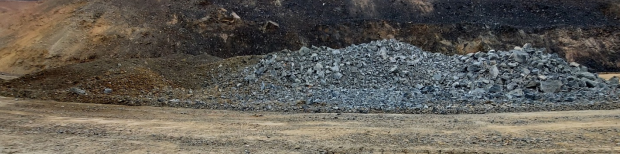
\includegraphics[width=0.8\textwidth]{media/gor/image31}
	\caption*{Рис. 4 -- Качество взрыва на визуальный осмотр}
\end{figure}
\begin{multicols}{2}


{\bfseries Результаты и обсуждение.} Результаты исследования показали, что
использование программы Micromine позволило значительно улучшить
параметры дробления руды. В частности, экспериментальный блок 270\_007
продемонстрировал успешные результаты, которые были достигнуты благодаря
корректировке параметров БВР на основе расчетов линии наименьшего
сопротивления. Сравнение с результатами, полученными без использования
геотехнических данных, показало следующие изменения:

- Общее количество скважин уменьшилось на 19 единиц.

- Объем буровых работ сократился на 102,4 п.м., что указывает на
повышение эффективности использования ресурсов.

- Выход горной массы на одну скважину увеличился на 1,5 п.м./скв., что
свидетельствует о более эффективном дроблении руды.

Таким образом, использование программы Micromine способствовало
улучшению основных параметров буровзрывных работ, несмотря на отсутствие
полноценной блочной модели (рисунок 4).


Четко видно границу литологии, так же отсутствуют некондиционные куски
горной массы в частях блока, где применялась расширенная сетка бурения.

Преимущества исследования включают оптимизацию сетки бурения и снижение
объемов буровых работ, что подтверждает эффективность выбранного
подхода. Однако следует критически рассмотреть и возможные недостатки,
такие как ограниченность применения методов без полноценной
литологической модели и несовместимость с другим ПО, что могло повлиять
на точность моделирования.

{\bfseries Выводы.} В ходе исследования была продемонстрирована
эффективность программы Micromine в улучшении параметров дробления руды
при скважинном бурении. Несмотря на отсутствие литологической блочной
модели и несовместимость с ShotPlus, Micromine позволила разработать
альтернативный подход к буровзрывным работам. Оптимизация сетки бурения
и расчеты линии наименьшего сопротивления способствовали снижению
количества скважин и объема буровых работ, повышая общую эффективность.
Программа также учитывала геомеханические и геологические особенности,
что улучшило стабильность подачи материала и соответствие экологическим
нормам.
\end{multicols}


\begin{center}
{\bfseries Литература}
\end{center}
\begin{references}

1.Malanchuk Z.R., Fedotenko V.S., E. Aben, Orynbaev B.A. Improving
efficiency of rock breaking using pre-weakening of rock mass//Eurasian
Mining.- 2023.-Vol.40(2).-P. 62-65 \linebreak DOI 10.17580/em.2023.02.13

2.Мельниченко И.А., Кожухов А.А., Омельченко Д.Р., Мосейкин В.В.
Построение трехмерной модели месторождения с использованием принципов
блочного моделирования и искусственных нейронных сетей// Горный
информационно-аналитический бюллетень.-2022.-№ 10.-С.5-19. \linebreak DOI
10.25018/0236\_1493\_2022\_10\_0\_5

3. Федорова С.В., Кожевников Д.Н. Информационные технологии в горном
деле //XXI ВЕК. Техносферная безопасность.-2024.- №9(3).- С.216-224.
\href{http://dx.doi.org/10.21285/2500-1582-2024-9-3-216-224}{DOI
10.21285/2500-1582-2024-9-3-216-224}

4. Modis, K., Valakas, G., \& Sideri, D. (2023). Geostatistics and Ore
Reserves Estimation {[}Undergraduate textbook{]}. Kallipos, Open
Academic Editions.
\href{http://dx.doi.org/10.57713/kallipos-203}{DOI10.57713/kallipos-203}

5.Wellmann, Florian \& Caumon, Guillaume. (2018). Chapter One-3-D
Structural geological models: \linebreak Concepts, methods, and uncertainties//\href{https://www.sciencedirect.com/bookseries/advances-in-geophysics}{Advances
in Geophysics}.-2018.-\href{https://www.sciencedirect.com/bookseries/advances-in-geophysics/vol/59/suppl/C}{Vol.
59}.~- P. 1-121. 

\href{http://dx.doi.org/10.1016/bs.agph.2018.09.001}{DOI
10.1016/bs.agph.2018.09.001} 

6.Лесонен М. В., Сень М. С. Использование блочной модели для
технико-экономической оценки месторождений ТПИ (на примере открытого
способа отработки) // Экономика. -2010. - С. 85--86.

7. Шульга Е.С. Чем порадует 2018 год пользователей программы Micromine
// Золото и технологии. -2017. - № 4 (38).- С. 50--53.

8. Д.К. Ахметканов, Л.Е. Тян, Е.Х. Абен, М. Елузах Оптимизация
численности и качественных характеристик подземного выемочного
оборудования с применением программного обеспечения Micromine //Вестник
Казахский университет технологии и бизнеса. -Астана, 2024, - №2(23). -С.
420-428. DOI \href{https://doi.org/10.58805/kazutb.v.2.23-319}{10.58805/kazutb.v.2.23-319}

9. Вохмин С.А., Курчин Г.С., Кирсанов А.К., Шкаруба Н.А. Расчёт
  параметров буровзрывных работ при строительстве подземных горных
  выработок. Монография. - Красноярск: Сибирский федеральный
  университет, 2022. -180 с. ISBN: 978-5-7638-4481-8

10. Разработка методики проектирования буровзрывных работ на открытых
  горных выработках с применением ГГИС Micromine. URL:
  {https://www.micromine.kz/2023-5-release/}

11. Катанов И.Б., Сысоев А.А. Буровзрывные работы на карьерах. Учебное
  пособие.   Издательство:\linebreak ~\href{https://www.labirint.ru/pubhouse/2357/}{Инфра-Инженерия},
  2021. -208 с. ISBN: 978-5-9729-0757-1 URL:{https://www.labirint.ru/books/807059/}

12. Игбаев Т.М., Ахметканов Д.К. Разрушение крепких пород зарядом
взрывчатого вещества каркасно-ступенчатого действия // Вестник Казахский
университет технологии и бизнеса.-2024.-№1(22).- С. 286-292. DOI
\href{https://doi.org/10.58805/kazutb.v.1.22-286}{10.58805/kazutb.v.1.22-286}

\end{references}

\begin{center}
{\bfseries References}
\end{center}

\begin{references}

1.Malanchuk Z.R., Fedotenko V.S., E. Aben, Orynbaev B.A. Improving
efficiency of rock breaking using pre-weakening of rock mass//Eurasian
Mining.- 2023.-Vol.40(2).-P. 62-65
\linebreak DOI 10.17580/em.2023.02.13

2.Mel' nichenko I.A., Kozhuhov A.A.,
Omel' chenko D.R., Mosejkin V.V. Postroenie trehmernoj modeli mestorozhdenija s
ispol' zovaniem principov blochnogo modelirovanija i
iskusstvennyh nejronnyh setej// Gornyj informacionno-analiticheskij
bjulleten'.-2022.-№ 10.-S.5-19. \linebreak DOI
10.25018/0236\_1493\_2022\_10\_0\_5. {[}in Russian{]}

3. Fedorova S.V., Kozhevnikov D.N. Informacionnye tehnologii v gornom
dele //XXI VEK. Tehnosfernaja bezopasnost'.-2024.-
№9(3).- S.216-224.
\linebreak DOI 10.21285/2500-1582-2024-9-3-216-224. {[}in Russian{]}

4. Modis, K., Valakas, G., \& Sideri, D. (2023). Geostatistics and Ore
Reserves Estimation {[}Undergraduate textbook{]}. Kallipos, Open
Academic Editions.
\href{http://dx.doi.org/10.57713/kallipos-203}{DOI10.57713/kallipos-203}

5.Wellmann, Florian \& Caumon, Guillaume. (2018). Chapter One-3-D
Structural geological models:\linebreak Concepts, methods, and
uncertainties//\href{https://www.sciencedirect.com/bookseries/advances-in-geophysics}{Advances
in Geophysics}.-2018. -\href{https://www.sciencedirect.com/bookseries/advances-in-geophysics/vol/59/suppl/C}{Vol.
59}.~- P. 1-121. \linebreak \href{http://dx.doi.org/10.1016/bs.agph.2018.09.001}{DOI
10.1016/bs.agph.2018.09.001} \hl{}

6.Lesonen M. V., Sen'{} M. S.
Ispol' zovanie blochnoj modeli dlja
tehniko-jekonomicheskoj ocenki \\mestorozhdenij TPI (na primere otkrytogo
sposoba otrabotki) // Jekonomika. -2010. - S. 85--86. {[}in Russian{]}

7. Shul' ga E.S. Chem poraduet 2018 god
pol' zovatelej programmy Micromine // Zoloto i
tehnologii. -2017. - № 4 (38).- S. 50--53. {[}in Russian{]}

8. D.K. Ahmetkanov, L.E. Tjan, E.H. Aben, M. Eluzah Optimizacija
chislennosti i kachestvennyh \linebreak harakteristik podzemnogo vyemochnogo
oborudovanija s primeneniem programmnogo obespechenija \linebreak Micromine
//Vestnik Kazahskij universitet tehnologii i biznesa. -Astana, 2024, -
№2(23). -S. 420-428. DOI 10.58805/kazutb.v.2.23-319. {[}in Russian{]}

9.Vohmin S.A., Kurchin G.S., Kirsanov A.K., Shkaruba N.A. Raschjot
parametrov burovzryvnyh rabot pri stroitel' stve
podzemnyh gornyh vyrabotok. Monografija. - Krasnojarsk: Sibirskij
federal' nyj universitet, 2022. -180 s. ISBN: 978-5-7638-4481-8. {[}in Russian{]}

10.Razrabotka metodiki proektirovanija burovzryvnyh rabot na otkrytyh
gornyh vyrabotkah s primeneniem GGIS Micromine. URL: https://www.micromine.kz/2023-5-release/{[}in Russian{]}

11.Katanov I.B., Sysoev A.A. Burovzryvnye raboty na
kar' erah. Uchebnoe posobie.
Izdatel' stvo: Infra-Inzhenerija, 2021. -208 s. ISBN:
978-5-9729-0757-1. URL: https://www.labirint.ru/books/807059/.{[}in Russian{]}

12.Igbaev T.M., Ahmetkanov D.K. Razrushenie krepkih porod zarjadom
vzryvchatogo veshhestva karkasno-stupenchatogo dejstvija // Vestnik
Kazahskij universitet tehnologii i biznesa.-2024.-№1(22).- S. 286-292.
DOI 10.58805/kazutb.v.1.22-286. {[}in Russian{]}
\end{references}
\begin{authorinfo}

\hspace{1em}\emph{{\bfseries Сведения об авторах}}

Қазбек А.Ә. -- магистрант Satbayev University, г.Алматы, Казахстан,
e-mail:
\href{mailto:Abulaikhan93@mail.ru}{\nolinkurl{Abulaikhan93@mail.ru}};

Ахметканов Д.К. -- канд.техн.наук, ассоциированный профессор, Satbayev
University, г.Алматы, Казахстан, \linebreak e-mail:
\href{mailto:d.akhmetkanov@satbayev.university}{\nolinkurl{d.akhmetkanov@satbayev.university}};

Абен Е.Х. - канд.техн.наук, ассоциированный профессор, Satbayev
University, г.Алматы, Казахстан, \linebreak e-mail:
\href{mailto:y.aben@satbayev.university}{\nolinkurl{y.aben@satbayev.university}};

Мырзахметов С.С. - канд.техн.наук, ассоциированный профессор, Satbayev
University, г.Алматы, Казахстан, \linebreak e-mail:
\href{mailto:s.myrzakhmetov@satbayev.university}{\nolinkurl{s.myrzakhmetov@satbayev.university}}.

\hspace{1em}\emph{{\bfseries Information about the authors}}

Kazybek A. -- undergraduate student Satbayev University, Almaty,
Kazakhstan, e-mail:
\href{mailto:Abulaikhan93@mail.ru}{\nolinkurl{Abulaikhan93@mail.ru}};

Akhmetkanov D. -- Candidate of Technical Sciences, Associate Professor
of Satbayev University, Almaty, Kazakhstan, e-mail:
\href{mailto:d.akhmetkanov@satbayev.university}{\nolinkurl{d.akhmetkanov@satbayev.university}};

Aben Y. -- Candidate of Technical Sciences, Associate Professor of
Satbayev University, Almaty, Kazakhstan, e-mail:
\linebreak \href{mailto:y.aben@satbayev.university}{\nolinkurl{y.aben@satbayev.university}};

Myrzakhmetov S. -- Candidate of Technical Sciences, Associate Professor
of Satbayev University, Almaty, Kazakhstan, e-mail:
\href{mailto:s.myrzakhmetov@satbayev.university}{\nolinkurl{s.myrzakhmetov@satbayev.university}}.
\end{authorinfo}
